\begin{figure}[h!]
\textbf{Tema d'Esame di Gennaio 2016}\\ \\
Una bottiglia (volume $V_B=1L$ e massa $100 g$) contiene $50$atm di $He$ (gas perfetto) a
temperatura ambiente. Calcolare la forza che bisogna esercitare verticalmente sulla bottiglia
per tenerla completamente immersa in acqua. Massa atomica $He= 6.64 \cdot 10^{24} g$. densità
acqua $1000 kg/m^3$.

\end{figure}

\begin{figure}[h!]
\textbf{Tema d'Esame di Febbraio 2016}\\ \\
Una conduttura di diametro costante scende da una montagna per un dislivello di $40m$. La pressione del fluido che scorre nella conduttura è di $1$atm nel punto più alto e $5$atm nel punto più basso. La velocità del fluido a monte è $5m/s$. Calcolare la densità del fluido.
\begin{center}
		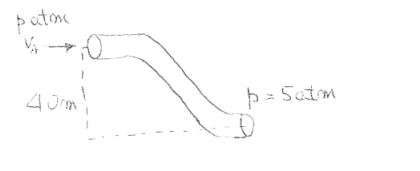
\includegraphics[scale=1.1]{ES4/FEB042016.jpg}
	\end{center}
\end{figure}

\begin{figure}[h!]
\textbf{Tema d'Esame di Giugno 2016}\\ \\
Un corpo sferico di massa $230 kg$ è immerso in acqua ($\rho_{H2O} = 1000kg/m^3 $). Il raggio del corpo
è $r = 0.07 m$. il corpo viene appeso ad un palloncino pieno d'elio ($\rho_{elio} = 0,17 kg/m3$ ) Calcolare il raggio minimo del palloncino per cui i due corpi non vadano a fondo; il palloncino è sferico e ha massa $85g$.
\begin{center}
		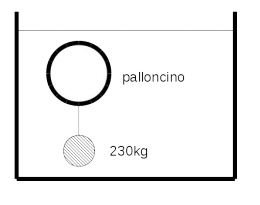
\includegraphics[scale=1.1]{ES4/GIU042016.jpg}
	\end{center}
\end{figure}

\begin{figure}[h!]
	\textbf{Tema d'Esame di Luglio 2016}\\ \\
	Un cilindro con un volume iniziale di $12$ litri contiene $23 g$ di ossigeno (peso
molecolare $A = 32 g/mol$) alla temperatura di $25^{\circ}C$. La temperatura viene portata a 35°C e il
volume ridotto a 8.5 litri. Qual'è la pressione finale del gas? Si assuma che il gas si comporti
come un gas perfetto.

	\begin{center}
			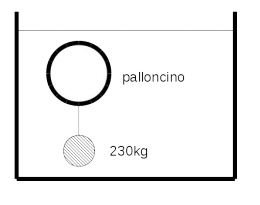
\includegraphics[scale=1.1]{ES4/GIU042016.jpg}
	\end{center}
\end{figure}